%&<tex>
\documentclass[notheorems,xcolor=dvipsnames]{beamer}
\usetheme{Rochester}
%\usefonttheme{serif}


%\usepackage[hmargin=2.5cm, vmargin=2cm]{geometry}
\usepackage{amssymb, mathtools, yhmath, graphicx}
\usepackage[most]{tcolorbox}
%\usepackage{fontspec, type1cm, titlesec, titling, fancyhdr, tabularx}
%\usepackage{unicode-math}
\usepackage{float}
\usepackage{transparent}
\usepackage[normalem]{ulem}
\usepackage{bm}

%\usepackage{eulervm}

\usepackage{xpatch}
\usepackage{relsize}
\usepackage{scalerel}
\usepackage{stackengine}
\usepackage{gauss}
%\usepackage[abbreviations, per-mode=symbol]{siunitx}
\usepackage[CheckSingle, CJKmath]{xeCJK}
\usefonttheme{professionalfonts}
\usepackage{ccfonts}
%\usepackage{CJKulem}
%\usepackage{enumitem}
\usepackage{tikz}
\usepackage{minted}
\setminted{fontsize=\footnotesize, linenos, frame=lines}
%\usemintedstyle{monokai}
%\usepackage{circuitikz}
%\setCJKmainfont[BoldFont=cwTex Q Hei]{cwTex Q Ming}
%\setCJKsansfont[BoldFont=cwTex Q Hei]{cwTex Q Ming}
%\setCJKmonofont[BoldFont=cwTex Q Hei]{cwTex Q Ming}
\setCJKmainfont{Source Han Sans TW}
\newfontfamily\SHSTW{Source Han Sans TW}

%\def\normalsize{\fontsize{12}{18}\selectfont}
%\def\large{\fontsize{14}{21}\selectfont}
%\def\Large{\fontsize{16}{24}\selectfont}
%\def\LARGE{\fontsize{18}{27}\selectfont}
%\def\huge{\fontsize{20}{30}\selectfont}

%\titleformat{\section}{\bf\Large}{\arabic{section}}{24pt}{}
%\titleformat{\subsection}{\large}{\arabic{subsection}.}{12pt}{}
%\titlespacing*{\subsection}{0pt}{0pt}{1.5ex}

%\usepackage{parskip}
%\parindent=24pt
%\parskip=1em

\makeatletter
\newcommand{\myRelbar}{%
    {\Rightarrow}%
    \llap{\color{white}{\rule[-0.2ex]{1.1ex}{2ex}}}%
    \kern-1.5ex}
\let\saveLongrightarrow\Longrightarrow
\newcommand{\Larr}{%
    \mathrel{\rlap{$\m@th\myRelbar\myRelbar$}%
    \phantom{{\saveLongrightarrow}}%
    \llap{$\m@th\Rightarrow$}}}

\renewcommand{\Longrightarrow}{%
    %%\mathrel{\rlap{$\m@th\myRelbar\myRelbar$}%
    %%\phantom{{\saveLongrightarrow}}%
    %%\llap{$\m@th\Rightarrow$}}}
\Relbar\joinrel\mathrel{\raisebox{0.095ex}{\scalebox{0.85}{${\Rightarrow}$}}}
}
\makeatother


\newcommand{\img}{\mathsf{i}}
\newcommand{\ex}{\mathsf{e}}
\newcommand{\dD}{\mathrm{d}}
\newcommand{\dI}{\,\mathrm{d}}

\newcommand\abs[1]{\left\lvert #1 \right\rvert}
\newcommand{\ord}{\mathcal{O}}
\newcommand*{\defeq}{\triangleq}
\renewcommand*{\sharp}{\mathlarger{\#}}
\newcommand*{\bZ}{\mathbb{Z}}
\newcommand*{\bF}{\mathbb{F}}
\newcommand*{\correspond}{\mathrel{\stackon[1.5pt]{=}{\stretchto{%
    \scalerel*[\widthof{=}]{\wedge}{\rule{1ex}{3ex}}}{0.5ex}}}}
\newcommand*{\Expect}{{\rm I\kern-.3em E}}

\theoremstyle{definition}
\newtheorem{theorem}{定理}
\newtheorem{lemma}{引理}
\newtheorem{problem}{例題}
\newtheorem{definition}{定義}

\newenvironment{missue}{%
\setbeamercolor{block title}{bg=ForestGreen,fg=white}
\setbeamercolor{block body}{bg=blue!20!green!20,fg=black}
\begin{block}{\centering 問題}}{\end{block}}

\newenvironment{exercise}{%
\setbeamercolor{block title}{bg=ForestGreen,fg=white}
\setbeamercolor{block body}{bg=blue!20!green!20,fg=black}
\begin{block}{習題}}{\end{block}}

\renewenvironment{proof}{%
\begin{tcolorbox}[frame empty] {\bf 證明:}\ }{\end{tcolorbox}}

\setbeamercovered{transparent}
%\usefonttheme[onlymath]{serif}
%\settowidth{\leftmargini}{\usebeamertemplate{itemize item}}

%\makeatletter
%\patchcmd\beamer@@tmpl@frametitle{\insertframetitle}{\insertsection-\insertframetitle}{}{}
%\makeatother

\title{IOI-camp lecture Math}
\author{Meteor}

\renewcommand*{\emph}[1]{{\bf #1}}

\begin{document}

\begin{frame}
  \titlepage
\end{frame}

\section{Introduction}

\begin{frame}{\secname}
  程式競賽中的數學:

  \begin{itemize}
    \setlength{\itemindent}{2em}
    \item<2-> 數學知識
    \item<3> 數學想法
  \end{itemize}
\end{frame}

\begin{frame}[t]{\secname \ -- 數學知識例子}
  \begin{problem}[平方國的平方幣, TIOJ 1349]
    給你一個正整數 $n$,請找出最小的 $k$,使得存在 $k$ 個平方數 $a_1^2, a_2^2, \cdots, a_k^2$
    使得 $\sum a_i^2 = n$ 。($n \leq 10^7$)
  \end{problem}

  \begin{itemize}
    \item<2-> 一個很極端的「結論題」。
    \item<3-> 所有正整數都可以寫成 $4$ 個平方數的和 (Lagrange 1770)。
    \item<4-> 太結論也不是很有趣……
  \end{itemize}
\end{frame}

\begin{frame}[t]{\secname \ -- 數學知識例子 2}
  \begin{problem}[Taxes, Codeforces 735D]%
    在一個很古怪的國家,如果你賺了 $x$ 元,你就要繳 $d$ 塊錢的稅,其中 $d$ 是 $x$ 的因數且小於
    $n$ 裡最大的一個。

    \medskip
    現在有一個人賺了 $n$ 元,他想把 $n$ 拆成 $n = n_1 + n_2 + \cdots + n_k$ 然後 $n_i$ 各自繳稅,
    請問他最多可以逃過多少稅?($n \leq 2 \times 10^9$)
  \end{problem}

  \begin{itemize}
    \item<2-> Goldbach's conjecture: 大於 $2$ 的偶數都可以寫成兩個質數的和。
  \end{itemize}
\end{frame}

\begin{frame}[t]{\secname \ -- 數學想法例子}
  但大部份還是屬於「數學想法」的問題。

  \pause
  \medskip
  \begin{problem}[2015 ICPC Daejeon regional pE]
    給你一堆數列 $a_1, a_2, \cdots, a_n$,你要找一個排列 $\sigma$,使得
    \[ \max \Big(
      \abs{a_{\sigma(1)} - a_{\sigma(2)}},
      \abs{a_{\sigma(2)} - a_{\sigma(3)}}, \cdots,
      \abs{a_{\sigma(n)} - a_{\sigma(1)}}
      \Big) \]
    最小。 ($n \leq 10^4$)
  \end{problem}

  \pause
  \begin{definition}
    一個大小為 $n$ 的\emph{排列}是一個從 $[1, n]$ 打到自己的一一對應函數。
  \end{definition}
\end{frame}

\begin{frame}[t]{\secname \ -- 數學想法例子}
  解題四部曲:
  \pause

  \begin{enumerate}[<+->]
    \item 嘗試、觀察:在計算紙上多試試
    \item 神猜結論
    \item {\color{gray} (稍微)}證明
    \item 寫 code
  \end{enumerate}
  \pause

  \bigskip
  亂講的,多半要臨機應變,見招拆招。
\end{frame}

\begin{frame}[t]{\secname \ -- 數學想法例子}
  \begin{enumerate}
    \item 嘗試、觀察
    \item 神猜結論
  \end{enumerate}
  \pause

  \begin{figure}
    \centering
    \only<+>{
    \begin{tikzpicture}[scale=0.8]
      \draw[-latex, thick] (0, 0) -- (10, 0);
      \foreach \x [count=\i] in {0.5, 2, 4, 6, 8} {
        \fill (\x, 0) node (\i) {} circle (1.5mm);
      }
      \node at (0, 0) {};
      \draw (1) edge[bend left=50, -latex, thick] (2);
      \draw (2) edge[bend left=50, -latex, thick] (3);
      \draw (3) edge[bend left=50, -latex, thick] (4);
      \draw (4) edge[bend left=50, -latex, thick] (5);
      \draw (5) edge[bend left=50, -latex, thick] (1);
      \node at (5, -3) {應該不是…};
    \end{tikzpicture}
    }

    \only<+>{
    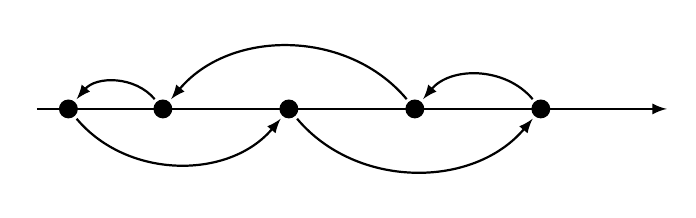
\begin{tikzpicture}[scale=0.8]
      \draw[-latex, thick] (0, 0) -- (10, 0);
      \foreach \x [count=\i] in {0.5, 2, 4, 6, 8} {
        \fill (\x, 0) node (\i) {} circle (1.5mm);
      }
      \node at (0, 0) {};
      \draw (2) edge[bend right=50, -latex, thick] (1);
      \draw (1) edge[bend right=50, -latex, thick] (3);
      \draw (3) edge[bend right=50, -latex, thick] (5);
      \draw (5) edge[bend right=50, -latex, thick] (4);
      \draw (4) edge[bend right=50, -latex, thick] (2);
    \end{tikzpicture}
    }

    \only<+>{
    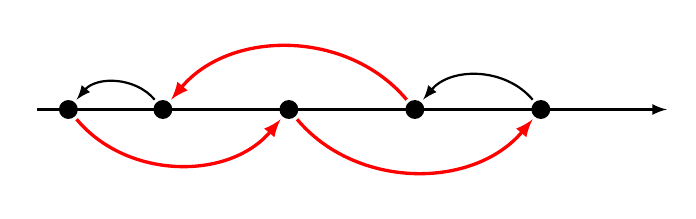
\begin{tikzpicture}[scale=0.8]
      \draw[-latex, thick] (0, 0) -- (10, 0);
      \foreach \x [count=\i] in {0.5, 2, 4, 6, 8} {
        \fill (\x, 0) node (\i) {} circle (1.5mm);
      }
      \node at (0, 0) {};
      \draw (2) edge[bend right=50, -latex, thick] (1);
      \draw (1) edge[bend right=50, -latex, very thick, red] (3);
      \draw (3) edge[bend right=50, -latex, very thick, red] (5);
      \draw (5) edge[bend right=50, -latex, thick] (4);
      \draw (4) edge[bend right=50, -latex, very thick, red] (2);
    \end{tikzpicture}
    }
  \end{figure}
\end{frame}

\begin{frame}[t]{\secname \ -- 數學想法例子}
  \begin{enumerate}
    \setcounter{enumi}{2}
    \item 證明
  \end{enumerate}

  \begin{figure}
    \centering
    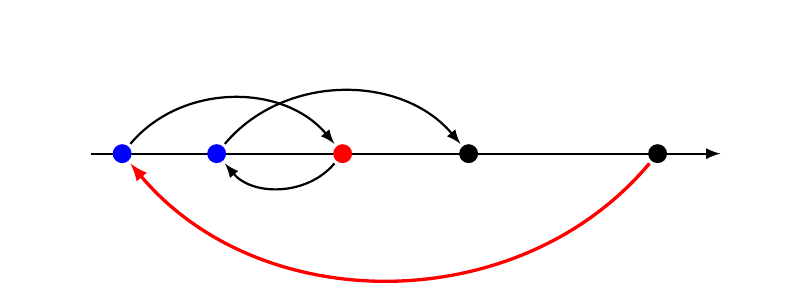
\begin{tikzpicture}[scale=0.8]
      \useasboundingbox (-1, -2) rectangle (11, 2);
      \draw[-latex, thick] (0, 0) -- (10, 0);
      \fill[red] (4, 0) node (1) {} circle (1.5mm);
      \fill (6, 0) node (2) {} circle (1.5mm);
      \fill<+-> (9, 0) node (3) {} circle (1.5mm);
      \fill<+->[blue] (2, 0) node (4) {} circle (1.5mm);
      \draw<.-> (1) edge[bend left=50, -latex, thick] (4);
      \draw<.-> (4) edge[bend left=50, -latex, thick] (2);
      \fill<+->[blue] (0.5, 0) node (5) {} circle (1.5mm);
      \draw<.-> (5) edge[bend left=50, -latex, thick] (1);
      \draw<.-> (3) edge[bend left=50, -latex, very thick, red] (5);
    \end{tikzpicture}
  \end{figure}
\end{frame}

\begin{frame}[t, fragile]{\secname \ -- 數學想法例子}
  \begin{enumerate}
    \setcounter{enumi}{3}
    \item 寫 code
  \end{enumerate}

  \begin{minted}{cpp}
sort(begin(a), end(a));
int ans = 0;
for (int i=0; i<n-2; i++)
  ans = max(ans, a[i+2] - a[i]);
cout << ans << endl;
  \end{minted}
  \pause

  \bigskip
  Very easy! --- 有時漂亮的結論就會有很短的程式碼。
\end{frame}

\begin{frame}{\secname}
  相同的題目就不會在出現第二次了。
  \pause

  \bigskip
  \alert{但用類似想法的題目有可能會在出現!}

  \pause
  \smallskip
  要有舉一反三的能力!
\end{frame}

\begin{frame}[t]{\secname \ -- 數學想法例子 2}
  \begin{problem}[2016 NTU PK pF]
    給你一堆數列 $a_1, a_2, \cdots, a_n$,你要找一個排列 $\sigma$,使得
    \[ \min_{1 \leq i < n} \abs{a_{\sigma(i)} - a_{\sigma(i+1)}} \]
    最大。 ($n \leq 2 \times 10^5$)
  \end{problem}
  \pause

  \medskip
  我們先想 $n$ 是\alert{偶數}的 case。
\end{frame}

\begin{frame}[t]{\secname \ -- 數學想法例子 2}
  \begin{enumerate}
    \item 嘗試、觀察
    \item 神猜結論
  \end{enumerate}

  \begin{figure}
    \centering
    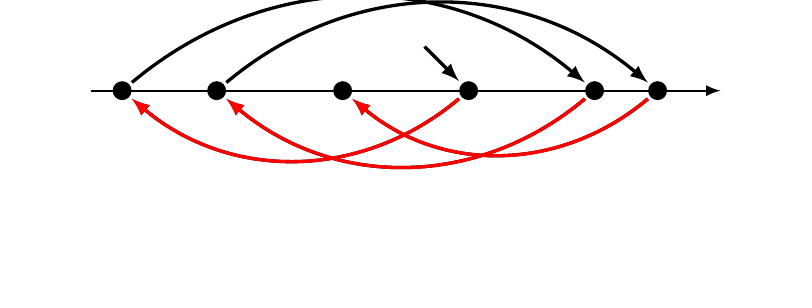
\begin{tikzpicture}[scale=0.8]
      \useasboundingbox (-1, -3) rectangle (11, 1);
      \draw<+->[-latex, thick] (0, 0) -- (10, 0);
      \foreach \x [count=\i] in {0.5, 2, 4, 6, 8, 9} {
        \fill (\x, 0) node (\i) {} circle (1.5mm);
      }
      \draw<+> (4) edge[bend left=40, -latex, very thick] (1);
      \draw<.-> (1) edge[bend left=40, -latex, very thick] (5);
      \draw<.> (5) edge[bend left=40, -latex, very thick] (2);
      \draw<.-> (2) edge[bend left=40, -latex, very thick] (6);
      \draw<.> (6) edge[bend left=40, -latex, very thick] (3);
      \draw<.-> (4) ++ (-0.7, 0.7) edge[-latex, very thick] (4);

      \draw<+-> (4) edge[bend left=40, -latex, very thick, red] (1);
      \draw<.-> (5) edge[bend left=40, -latex, very thick, red] (2);
      \draw<.-> (6) edge[bend left=40, -latex, very thick, red] (3);
    \end{tikzpicture}
  \end{figure}
\end{frame}

\begin{frame}[t]{\secname \ -- 數學想法例子 2}
  \begin{enumerate}
    \setcounter{enumi}{2}
    \item 證明
  \end{enumerate}

  \begin{figure}
    \centering
    \begin{tikzpicture}[scale=0.8]
      \useasboundingbox (-1, -3) rectangle (11, 1);
      \draw<+->[-latex, thick] (0, 0) -- (10, 0);
      \foreach \x [count=\i] in {0.5, 9} {
        \fill (\x, 0) node (\i) {} circle (1.5mm);
      }
      \foreach \x [count=\i] in {2, 4, 6, 8} {
        \fill[red] (\x, 0) node (\i) {} circle (1.5mm);
      }

      \draw[latex-latex] (2, -.5) -- (8, -.5);
      \draw (2, -.8) -- (2, -.2);
      \draw (8, -.8) -- (8, -.2);
    \end{tikzpicture}
  \end{figure}
\end{frame}

\begin{frame}{\secname \ -- 數學想法例子 2}
  \begin{exercise}
    請完成奇數的情況。
  \end{exercise}
\end{frame}

\section{數論}

\begin{frame}[t,fragile]{\secname}
  \begin{problem}[An Easy Problem, NTUJ 1423]
    給你等式 $a^b \equiv c \pmod{d}$ 中的其中 $3$ 個,請找出剩下的一個。
  \end{problem}
  \pause

  \bigskip
  \begin{enumerate}
    \item $a^b \equiv \raisebox{-.2mm}{\text{?}} \pmod{d}$: 快速冪,$\ord(\log b)$。
  \end{enumerate} \vspace{-1em} \pause
  \begin{minted}{cpp}
int fastpow(int a, int b, int m) {
    if (!b) return 1%m;
    int ret = fastpow(a*a%m, b/2, m);
    if (b&1) (ret *= a) %= m;
    return ret;
}
  \end{minted}
\end{frame}

\begin{frame}[t]{\secname}
  \begin{enumerate}
    \setcounter{enumi}{1}
    \item $a^b \equiv c \pmod{\text{?}}$ \pause $\implies \raisebox{-.2mm}{?} \mid a^b - c$ \pause
      \vspace{1em}
    \item<+-> $a^{\text{?}} \equiv c \pmod{p},\, p \text{ prime}$: $\ord\big( \sqrt{p} \big)$,有點難了。

      \[ a^{xk + y} \equiv c \pmod{p} \iff a^{xk} \equiv c a^{-y} \pmod{p} \]

      \begin{missue}<+->
        \centering
        怎麼求出 $a^{-y} \bmod p$?
      \end{missue}
  \end{enumerate}
\end{frame}

\begin{frame}{\secname}
  我們先離題一下。
  \pause

  \medskip
  數學上喜歡把東西抽象化,只留下「本質」,去掉多餘的東西。
  \pause

  \medskip
  \begin{missue}<+->
    \centering
    運算的「本質」是什麼?
  \end{missue}
\end{frame}

\begin{frame}{\secname \ -- 群}
\begin{definition}[群] 一個\emph{群}由一個集合 $G$ 和一個運算 $\cdot$ 構成,滿足
  \begin{itemize}
    \item 運算 $\cdot$ 是一個函數 $(G, G) \to G$,也就是說 $x \cdot y \in G$。
    \item 有\emph{結合律}:$(x \cdot y) \cdot z = x \cdot (y \cdot z)$
    \item 存在一個特別的元素 $1$ 叫作\emph{單位元},滿足 $1 \cdot x = x \cdot 1 = x$。
    \item 對每一個 $x$ 存在 $x^{-1} \in G$ 叫作\emph{反元素},滿足 $x \cdot x^{-1} = x^{-1} \cdot x = 1$。
  \end{itemize}
\end{definition}
\end{frame}

\begin{frame}[t]{\secname \ -- 群的例子}
  \begin{itemize}[<+->]
    \item 整數對於加法 $(\bZ, +)$ 是一個群。
    \item 旋轉是一個群,如 $0, \pi/2, \pi, 3\pi/2$。
    \item 模 $m$ 下的加法,寫作 $\bZ / m\bZ$。
    \item 一個元素生成的群 $\langle a \rangle \defeq \{ a^k \mid k \in \bZ \}$,我們把這種群叫作%
      \emph{循環群}。
  \end{itemize}

  \visible<+->{
  \begin{missue}
    \centering
    模 $m$ 下的乘法 $(\bZ / m\bZ)^{\times}$ 是一個群嗎?
  \end{missue}
  }
\end{frame}

\begin{frame}[t]{\secname \ -- $(\bZ / m\bZ)^{\times}$}
  剛剛那樣問並不精確,關鍵應是模 $m$ 下哪些元素有反元素?\pause

  \medskip
  $2$ 在模 $12$ 下就沒有反元素。 \pause

  \[ xy \equiv 1 \pmod{m} \pause\implies xy = mt' + 1 \pause\implies xy + mt = 1 \]

  \begin{missue}<+->
    \centering
    給定 $a, b, c$,$ax + by = c$ 什麼時候有整數解 $(x, y)$?
  \end{missue}
\end{frame}

\begin{frame}[t, fragile]{\secname \ -- $ax + by = c$}
  \begin{theorem} \vspace{-1em}
    \[a \bZ + b \bZ = \gcd(a, b) \bZ \]
  \end{theorem}\pause

  $a \bZ + b \bZ \supseteq \gcd(a, b) \bZ $:
  \begin{minted}{cpp}
pair<int, int> extend_gcd(int a, int b) {
    if(b == 0) return {1, 0};
    else {
        int k = a/b;
        pair<int, int> xy = gcd(b, a%b);
        return {xy.second, xy.first - k * xy.second};
    }
}
  \end{minted}
\end{frame}

\begin{frame}[t]{\secname \ -- $(\bZ / m\bZ)^{\times}$}
  \begin{lemma} \vspace{-1em}
    \[ x \in (\bZ / m\bZ)^{\times} \iff \gcd(x, m) = 1 \]
  \end{lemma}
  \pause

  \begin{proof}
    \begin{align*}
      \only<2->{xy \equiv 1 \ (\mathrm{mod}\ m) \text{ 有解} & \iff xy + mt = 1 \text{ 有解} \\}
      \only<3->{& \iff \gcd(x, m) = 1}
    \end{align*}
  \end{proof}
\end{frame}

\begin{frame}[t]{\secname \ -- $(\bZ / m\bZ)^{\times}$}
  \begin{missue}
    $(\bZ / m\bZ)^{\times}$ 有多少元素?也就是 $[1, n]$ 中有幾個數和 $n$ 互質?
  \end{missue}
  \pause

  \begin{theorem}[Euler $\varphi$ 函數]
    $\varphi(n)$ 表示 $[1, n]$ 有幾個數和 $n$ 互質,則如果 $n = p_1^{\alpha_1} p_2^{\alpha_2} \cdots p_k^{\alpha_k}$,則
    \[ \varphi(n)
      = n \left( 1 - \frac1{p_1} \right) \left( 1 - \frac1{p_2} \right) \cdots \left( 1 - \frac1{p_k} \right)\]
  \end{theorem}

\end{frame}

\begin{frame}[t]{\secname \ -- 子群}
  \begin{definition}
    如果 $H \subseteq G$ 且 $H$ 中任兩個元素的乘積、任一個元素的反元素還在 $H$ 裡,我們就說 $H$ 是 $G$ 的\emph{子群}。
  \end{definition}

  \begin{itemize}
    \item 所有偶數 $2 \bZ$ 對於加法是 $\bZ$ 的子群。
    \item $H \defeq \{\bar{1}, \bar2, \bar4\}$ 對於乘法是 $\bZ / 7\bZ$ 的子群。
  \end{itemize}
\end{frame}

\begin{frame}[t]{\secname \ -- Lagrange's Theorem}
  \begin{theorem}[Lagrange's theorem]
    如果 $H$ 是 $G$ 的子群,則 $\abs{G} = \abs{G / H} \abs{H}$,因此有 $\abs{H} \bigm\vert \abs{G}$。
  \end{theorem}
  \pause

  \bigskip
  \begin{theorem}[Euler's theorem] \vspace{-1em}
    \[ a^{\varphi(m)} \equiv 1 \pmod{m} \]
  \end{theorem}
\end{frame}

\begin{frame}[t]{{\secname} -- Euler's Theorem}
  \begin{proof} \\
    如果 $n$ 是最小的正整數使得 $a^n \equiv 1 \pmod{m}$,那
    $H \defeq \langle a \rangle = \{1, a, a^2, \cdots, a^{n-1}\}$ 有 $n$ 個元素。

    \smallskip
    由 Lagrange's theorem,$n \bigm\vert \abs{(\bZ / m\bZ)^{\times}} = \varphi(m)$,可令 $\varphi(m) = nk$,
    因此 $a^{\varphi(m)} = a^{nk} \equiv 1 \pmod{m}$。
  \end{proof}

  \begin{lemma}<+->
    \vspace{-1em}
    \[ \gcd(a, m) = 1 \implies a^{-1} \equiv a^{\varphi(m)-1} \pmod{m} \]
  \end{lemma}
\end{frame}

\begin{frame}{{\secname} -- Tonelli-Shanks algorithm}
  回到一開始的題目:
  \begin{enumerate}
    \setcounter{enumi}{3}
    \item $\raisebox{-.2mm}{\text{?}}^{b} \equiv c \pmod{p},\, p \text{ prime}$。
  \end{enumerate}
  \pause

  \bigskip
  先看 $b = 2$ 的情況。
  \begin{problem}[Square Roots in a Finite Group, 2013 大專院校 pJ]
    給定一個質數 $p$ 和 $a$,請求出 $x^2 \equiv a \pmod{p}$ 的解 $x$ 或輸出無解。
    ($a, p < 2^{31}$)
  \end{problem}
\end{frame}

\begin{frame}[t]{{\secname} -- Tonelli-Shanks algorithm}
  當時這一題有給一個小題示。

  \begin{enumerate}
    \item 把 $p-1$ 寫作 $p-1 = 2^s m$,其中 $m$ 是奇數。
    \item 找一個 $b$ 使得 $x^2 \equiv b \pmod{p}$ 無解。
    \item 令 $b \gets b^m,\, x \gets a^{(m+1)/2},\, t \gets a^m$,\\
      可以驗證 $x^2 \equiv at \pmod{p}$。
    \item 想辦法把 $t$ 調成 $1$ 你就獲勝了。
  \end{enumerate}
  \pause

  \begin{figure}
    \centering
    \includegraphics[width=0.45\textwidth]{figure/what.jpg}<+->
  \end{figure}
\end{frame}

\begin{frame}{{\secname} -- 原根}
  要有一點先備知識。\pause

  \bigskip
  \begin{theorem}
    \vspace{-1em}
    \[ (\bZ / m\bZ)^{\times} \text{ 是一個循環群} \iff m = 1, 2, 4, p^k, 2p^k \]
  \end{theorem}
  \pause

  \bigskip
  \begin{definition}
    如果 $(\bZ / m\bZ)^{\times} = \langle a \rangle$,我們就說 $a$ 是模 $m$ 下的\emph{原根}。
  \end{definition}
\end{frame}

\begin{frame}{{\secname} -- 原根}
  舉個例子,$m = 11, a = 2$。
  \begin{table}
    \begin{tabular}{c||c|c|c|c|c|c|c|c|c|c}
      $\bZ / 10\bZ$
      & 0 & 1 & 2 & 3 & 4 & 5 & 6 & 7 & 8 & 9 \\
      \hline
      $(\bZ / 11\bZ)^{\times}$
      & 1 & 2 & 4 & 8 & 5 & 10 & 9 & 7 & 3 & 6 \\
    \end{tabular}
  \end{table}
  \pause

  \[
    \begin{array}{cccccl}
      2 & +      & 4 & \equiv & 6 & \pmod{10} \\
      \updownarrow & & \updownarrow & & \updownarrow & \\
      4 & \times & 5 & \equiv & 9 & \pmod{11} \\
    \end{array}
  \]
  \pause

  可定義 $\log_a$,如 $\log_2(9) = 6$。
\end{frame}

\begin{frame}{{\secname} -- Tonelli-Shanks algorithm}
  $p = 25,\ p-1 = 2^s \cdot m = 2^3 \cdot 3$ \\
  \visible<2->{ $\log(t) = \log(a^m) = m \log(a)$。}\visible<3->{如果 $x \gets b$,那 $t \gets b^2$。}
  \begin{figure}
    \centering
    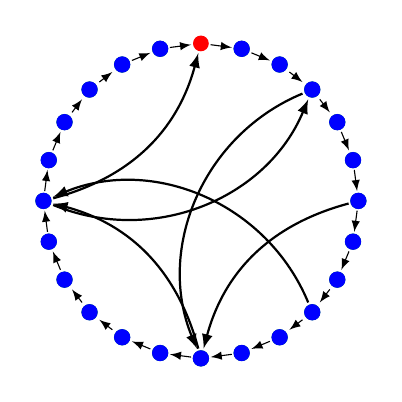
\begin{tikzpicture}
      \useasboundingbox (-2.2cm, -2.2cm) rectangle (2.2cm, 2.2cm);
      \fill[red] (90:2cm) node(0){} circle (1mm);
      \foreach \deg [count=\xi] in {75, 60,..., -255} {
        \fill (\deg:2cm) node(\xi){} circle (1mm);
        \pgfmathtruncatemacro{\hao}{mod(\xi,3)}
        \ifthenelse{\hao = 0}{
          \fill<2-5>[green] (\deg:2cm) node{} circle (1.02mm);
        }{ }
        \pgfmathtruncatemacro{\tsan}{mod(\xi,6)}
        \ifthenelse{\tsan = 0}{
          \fill<3-5>[blue] (\deg:2cm) node{} circle (1.04mm);
        }{ }
      }
      \foreach \xi [remember=\xi as \lastx (initially 0)] in {1,...,23}{ \draw[-latex] (\lastx) -- (\xi); }
      \draw[-latex] (23) -- (0);

      \foreach \xi [remember=\xi as \lastx (initially 6)] in {12, 18, 0} {
        \draw<4> (\lastx) edge[bend right, -latex, thick] (\xi);
      }

      \foreach \xi [remember=\xi as \lastx (initially 9)] in {18, 3, 12} {
        \draw<5> (\lastx) edge[bend right=45, -latex, thick] (\xi);
      }
    \end{tikzpicture}
  \end{figure}
\end{frame}

\begin{frame}[fragile]{{\secname} -- Tonelli-Shanks algorithm}
  \begin{minted}{cpp}
while (t != 1) {
    int k = 0, tp = t, tb = b;
    while (tp != 1) tp = (tp * tp) % p, k++;
    for (int i=0; i<s-k-1; i++) tb = (tb * tb) % p;
    x = x * tb % p;
    t = t * tb * tb % p;
}
  \end{minted}

\begin{exercise}
  把剩下的細節弄清楚!
\end{exercise}
\end{frame}

\section{Burnside's lemma}

\begin{frame}{{\secname}}
  \begin{problem}
    用 $M$ 種寶石可以做出多少 $N$ 個寶石的項鍊,假設旋轉相同視為相同。
  \end{problem}

  \begin{figure}
    \centering
    \begin{tikzpicture}
      \fill[red] (90:1cm) node(0){} circle (1mm);
      \fill[blue] (135:1cm) node(1){} circle (1mm);
      \fill[red] (180:1cm) node(2){} circle (1mm);
      \fill[red] (225:1cm) node(3){} circle (1mm);
      \fill[blue] (270:1cm) node(4){} circle (1mm);
      \fill[red] (-45:1cm) node(5){} circle (1mm);
      \fill[blue] (0:1cm) node(6){} circle (1mm);
      \fill[red] (45:1cm) node(7){} circle (1mm);
      \foreach \xi [remember=\xi as \lastx (initially 0)] in {1,2,...,7}{
        \draw[-] (\lastx) edge[bend right=22.5] (\xi); }
      \draw[-] (7) edge[bend right=22.5] (0);

      \node at (2, 0) {$\stackrel{\curvearrowleft}{=\joinrel=}$};

      \fill[red] (4, 0) ++ (90:1cm) node(0){} circle (1mm);
      \fill[red](4, 0) ++  (135:1cm) node(1){} circle (1mm);
      \fill[blue] (4, 0) ++ (180:1cm) node(2){} circle (1mm);
      \fill[red] (4, 0) ++ (225:1cm) node(3){} circle (1mm);
      \fill[red](4, 0) ++  (270:1cm) node(4){} circle (1mm);
      \fill[blue] (4, 0) ++ (-45:1cm) node(5){} circle (1mm);
      \fill[red](4, 0) ++  (0:1cm) node(6){} circle (1mm);
      \fill[blue] (4, 0) ++ (45:1cm) node(7){} circle (1mm);
      \foreach \xi [remember=\xi as \lastx (initially 0)] in {1,2,...,7}{
        \draw[-] (\lastx) edge[bend right=22.5] (\xi); }
      \draw[-] (7) edge[bend right=22.5] (0);
    \end{tikzpicture}
  \end{figure}
\end{frame}

\begin{frame}{{\secname} -- 問題的數學描述}
  \begin{itemize}[<+->]
    \item 旋轉會構成一個群 $G \defeq \langle g \rangle$。
    \item 物品(項鍊)會構成一個集合 $X$。
    \item 用 $G$ 把 $X$ 分門別類,寫作 $X / G$。
  \end{itemize}
\end{frame}

\begin{frame}{{\secname} -- 一些定義}
\begin{definition}
假設 $X$ 是一個集合,我們說 $G$ 透過一個運算 $\cdot$ 作用在 $X$ 上,如果以下三點成立:\pause
\begin{enumerate}[<+->]
  \item $g \cdot x \in X$。
  \item $(gh) \cdot x = g \cdot (hx)$。
  \item 如果 $1$ 是 $G$ 的單位元,則 $1 \cdot x = x$。
\end{enumerate}
\end{definition}
\end{frame}

\begin{frame}{{\secname} -- 再一些定義}
\begin{definition}
\begin{enumerate}[<+->]
  \item $G_x \defeq \{ g \in G : g x = x \}$,也就是固定 $x$ 下,所有不會動到 $x$ 的作用。
  \item $X^g \defeq \{ x \in X : g x = x \}$,也就是固定一個作用 $g$ 下的\emph{不動點}。
  \item $G x \defeq \{ gx : g \in G \}$,也被稱作是 $x$ 在 $G$ 下的\emph{軌道}。
  \item $X / G \defeq \{ Gx : x \in X \}$,也就是 $X$ 在 $G$ 下所有的軌道。
\end{enumerate}
\end{definition}
\end{frame}

\begin{frame}{{\secname}}
  \begin{theorem}[Burnside's lemma] \vspace{-1em}
  \[ \abs{X / G} = \frac{1}{\abs{G}} \sum_{g \in G} \abs{X^g} \]
  \end{theorem}\pause

  \medskip
  也就是說把每一個旋轉下的不動點加起來,除以旋轉的數量,就是種類數!
\end{frame}

\begin{frame}{{\secname} -- 證明}
  \begin{proof}
  \begin{align*}
   \frac{1}{\abs{G}} \sum_{g \in G} \abs{X^g} &= \frac{1}{\abs{G}}
   \sharp \big\{ (x, g) \mid x \in X, g \in G, x g = g \big\} \\
   &= \frac{1}{\abs{G}} \sum_{x \in X} \abs{G_x} \\
   &\stackrel{(1)}{=} \frac{1}{\abs{G}} \sum_{x \in X} \frac{\abs{G}}{\abs{Gx}}\\
   &\stackrel{(2)}{=} \sum_{Gx \in X / G} \ \sum_{x \in Gx} \frac{1}{\abs{Gx}} = \sum_{Gx \in X/G} 1\\
   &= \abs{X / G}
  \end{align*}
  \end{proof}
\end{frame}

\begin{frame}{{\secname} -- 證明}

  {\bf 關鍵:}
  \begin{enumerate}
    \item $\abs{G} = \abs{Gx} \abs{G_x}$
      \vspace{1em}
    \item $X = \bigsqcup_{Gx \in G/X} Gx$
  \end{enumerate}
\end{frame}

\begin{frame}[t]{{\secname} -- 應用}

  回到原本的例題,現在我們要算每個旋轉 $g$ 下的不動點 $X^g$。\pause

  \medskip
  \alert{注意:}不是只有 $\curvearrowleft$ 而已,有 $1, \curvearrowleft, \curvearrowleft^2, \cdots$。
  \pause

  \bigskip
  \begin{missue}
    如果今天在平面上旋轉 $\pi/2$ 和對 $x$ 軸鏡射要視為相同,要考慮哪些旋轉?
  \end{missue}
\end{frame}

\begin{frame}{{\secname} -- 應用}
  哪些項鍊是旋轉 $\curvearrowleft^k$ 下的不動點?有幾個觀察: \pause

  \medskip
  \begin{enumerate}
    \item 首先注意到 $X^{\curvearrowleft^k} = X^{\curvearrowleft^{\gcd(k, N)}}$
  \end{enumerate}
  \pause

  \begin{figure}
    \centering
    \begin{tikzpicture}
      \foreach \deg [count=\xi from 0] in {90, 114,..., 436} {
        \pgfmathtruncatemacro{\hao}{mod(\xi,3)}
        \ifthenelse{\hao = 0}{
          \fill[black] (\deg:1.5cm) node(\xi){} circle (1mm);
        }{
          \ifthenelse{\hao = 1}{
            \fill[blue] (\deg:1.5cm) node(\xi){} circle (1mm);
          }{
            \fill[red] (\deg:1.5cm) node(\xi){} circle (1mm);
          }
        }
      }
      \foreach \x [remember=\xi as \lastx (initially 0)] in {3, 6, ..., 15} {
        \pgfmathtruncatemacro{\xi}{mod(\x, 15)}
        \draw (\lastx) edge[bend left=40, thick, -latex] (\xi);
      }
      \node at (0, -2cm) {\footnotesize $k = 3$};
    \end{tikzpicture} \hspace*{1.5cm}
    \begin{tikzpicture}
      \foreach \deg [count=\xi from 0] in {90, 114,..., 436} {
        \pgfmathtruncatemacro{\hao}{mod(\xi,3)}
        \ifthenelse{\hao = 0}{
          \fill[black] (\deg:1.5cm) node(\xi){} circle (1mm);
        }{
          \ifthenelse{\hao = 1}{
            \fill[blue] (\deg:1.5cm) node(\xi){} circle (1mm);
          }{
            \fill[red] (\deg:1.5cm) node(\xi){} circle (1mm);
          }
        }
      }
      \foreach \x [remember=\xi as \lastx (initially 0)] in {9, 18, ..., 45} {
        \pgfmathtruncatemacro{\xi}{mod(\x, 15)}
        \draw (\lastx) edge[bend left=30, thick, -latex] (\xi);
      }
      \node at (0, -2cm) {\footnotesize $k = 9$};
    \end{tikzpicture}
    \caption{$n = 15$}
  \end{figure}
\end{frame}

\begin{frame}[t]{{\secname} -- 應用}
  \begin{enumerate}
    \setcounter{enumi}{1}
    \item 如果 $d \defeq \gcd(k, N)$,則
      \[ \abs{X^{\curvearrowleft^k}} = \abs{X^{\curvearrowleft^{\gcd(k, N)}}} = M^{d} \]
    \item 用 Burnside's lemma 得出
      \[ \abs{X / G} = \sum_{d \mid N} \sharp \{ k \mid \gcd(k, N) = d \} M^{d} \]
  \end{enumerate}
  \pause

  \begin{missue}
    對於 $d \mid N$ 的 $d$,$\sharp \{ k \mid \gcd(k, N) = d \}$ 如何求?
  \end{missue}
\end{frame}

\begin{frame}{{\secname} -- 應用}
  因為 $d \mid N$,
  \[ \sharp \{ k \mid \gcd(k, N) = d \} = \sharp \{ k \mid \gcd(k, N/d) = 1 \} = \varphi(N/d) \]
  \pause

  \bigskip
  總結答案:
  \[\sum_{d \mid N} \varphi(N/d) M^{d} \]

\end{frame}

\section{\texttt{C++17}}

\begin{frame}{{\secname}}
  \centering
  \Large
  \texttt{C++17} Features 分享!
\end{frame}

\begin{frame}[fragile]{{\secname}}
  \begin{itemize}[<+->]
    \setlength{\itemsep}{3mm}
    \item Class template deduction
      \begin{minted}[linenos=false]{cpp}
pair pr("hao"s, 123);
      \end{minted}
    \item Structure bindings
      \begin{minted}[linenos=false]{cpp}
auto [a, b] = pair("hao"s, 123);
      \end{minted}
    \item Initializers in \texttt{if}
      \begin{minted}[linenos=false]{cpp}
if (int x = fun(); x > 3) { ... }
      \end{minted}
    \item \texttt{std::clamp}
      \begin{minted}[linenos=false]{cpp}
assert(clamp(a, low, high) == min(max(a, low), high));
      \end{minted}
  \end{itemize}
\end{frame}

\section{線性代數}

\begin{frame}{\sout{組合賽局}~{\secname}}
  我們先看一題遊戲題。
  \begin{problem}[Takeover Wars, ACM-ICPC World Final pL]
    \small
    兩個人玩一個遊戲,A 有 $a_1, a_2, \cdots, a_k$ 個數字,B 有 $b_1, b_2, \cdots, b_h$ 個數字。
    由 A 先開始行動,每次行動可以選一個進行:
    \begin{enumerate}
      \item 融合:選兩個自己的數字 $x, y$,把 $x, y$ 拿掉換成 $x+y$。
      \item 吃掉:選一個自己的數字 $x$ 和對方的數字 $y$,如果 $x > y$,可以把 $y$ 拿掉。
      \item {\SHSTW 喵 PASS ~ヽ(`・д・´)}
    \end{enumerate}
    誰沒有數字了就輸了,問誰會贏? ($k, h \leq 10^5$)
  \end{problem} \pause

  有些題目沒想出來看到結論會氣死…
\end{frame}

\begin{frame}{{\secname} -- 例題}
  再看一題遊戲題。\pause

  \begin{problem}[Game on Bipartite Graph, {\small 2015-2016 Saratov SU Contest}]
  給一個二分圖 $G$ 和一個起點 $v$,兩人玩一個遊戲:輪流選一條和現在的點 $v$ 相鄰的邊 $(v, u)$,
  並沿著這條邊走到 $u$。走過的邊就不能再走了,誰沒有辦法再走就輸了。問你先手贏還是後手贏。($\abs{V} \leq 100$)
  \end{problem}
\end{frame}

\begin{frame}{{\secname} -- 例題}
  假設二分圖的兩個點集是 $X, Y$ 每個人在他的回合一定是固定從某個點集出發。\pause

  \medskip
  想一想後手什麼時候會贏?

  \medskip
  \begin{figure}
    \centering
    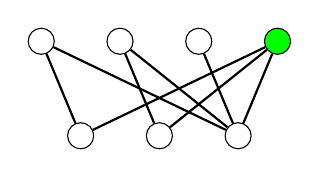
\begin{tikzpicture}[every node/.style={circle, draw}]
      \node[minimum width=3mm] (1) at (0, 0) {};
      \node[minimum width=3mm] (2) at (1, 0) {};
      \node[minimum width=3mm] (3) at (2, 0) {};
      \node[minimum width=3mm] (4) at (-.5, 1.2) {};
      \node[minimum width=3mm] (5) at (.5, 1.2) {};
      \node[minimum width=3mm] (6) at (1.5, 1.2) {};
      \node[minimum width=3mm, fill=green] (7) at (2.5, 1.2) {};

      \draw[thick] (1) edge (4);
      \draw[thick] (1) edge (7);
      \draw[thick] (2) edge (5);
      \draw[thick] (2) edge (7);
      \draw[thick] (3) edge (4);
      \draw[thick] (3) edge (5);
      \draw[thick] (3) edge (6);
      \draw[thick] (3) edge (7);
    \end{tikzpicture}
  \end{figure}
\end{frame}

\begin{frame}{{\secname} -- 例題}
  假設二分圖的兩個點集是 $X, Y$ 每個人在他的回合一定是固定從某個點集出發。
  不妨假設先手出發的是 $X$。\pause

  \medskip
  想一想後手什麼時候會贏?

  \medskip
  \begin{figure}
    \centering
    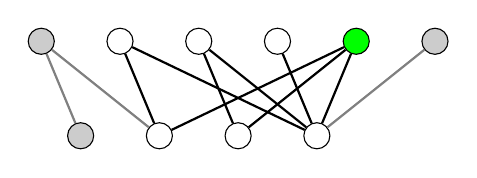
\begin{tikzpicture}[every node/.style={circle, draw}]
      \node[minimum width=3mm] (1) at (0, 0) {};
      \node[minimum width=3mm] (2) at (1, 0) {};
      \node[minimum width=3mm] (3) at (2, 0) {};
      \node[minimum width=3mm] (4) at (-.5, 1.2) {};
      \node[minimum width=3mm] (5) at (.5, 1.2) {};
      \node[minimum width=3mm] (6) at (1.5, 1.2) {};
      \node[minimum width=3mm, fill=green] (7) at (2.5, 1.2) {};
      \node<3>[fill=black!20, minimum width=3mm] (8) at (3.5, 1.2) {};
      \node<3>[fill=black!20, minimum width=3mm] (9) at (-1.5, 1.2) {};
      \node<3>[fill=black!20, minimum width=3mm] (0) at (-1, 0) {};

      \draw[thick] (1) edge (4);
      \draw[thick] (1) edge (7);
      \draw[thick] (2) edge (5);
      \draw[thick] (2) edge (7);
      \draw[thick] (3) edge (4);
      \draw[thick] (3) edge (5);
      \draw[thick] (3) edge (6);
      \draw[thick] (3) edge (7);

      \draw<3>[thick, black!50] (1) edge (9);
      \draw<3>[thick, black!50] (9) edge (0);
      \draw<3>[thick, black!50] (3) edge (8);
    \end{tikzpicture}
  \end{figure}
\end{frame}

\begin{frame}{{\secname} -- 例題}
  現在對於 $X$ 的第 $i$ 個點,如果他連到下面 $i_1, i_2, \cdots, i_k$ 個點,就令
  $\bm{v}_i = \sum 2^{i_t}$。\pause

  \medskip
  從剛才的討論可以知道如果存在 $\bm{v}_{j_1}, \bm{v}_{j_2}, \cdots, \bm{v}_{j_m}$ 使得
  \[ \bm{v}_s \in \{j_t\} \quad\text{且}\quad  \bm{v}_{i_1} \oplus \bm{v}_{i_2} \oplus \ldots \oplus \bm{v}_{i_m} \]
  則後手會贏。\pause

  \begin{missue}
    \begin{enumerate}
      \item 怎麼找 $j_1, j_2, \cdots, j_m$?
      \item 這個條件是否也是\emph{必要條件}?
    \end{enumerate}
  \end{missue}
\end{frame}

\begin{frame}{{\secname} -- 例題}
  這些 $\bm{v}_i$ 其實可以看作是 $\bF_2^n$ 向量空間中的向量,其中 $n \defeq \abs{Y}$。
  即 $1 \correspond (1, 0, 0, \cdots, 0),\ 2 \correspond (0, 1, 0, \cdots, 0)$ 等等。\pause

  \bigskip
  而條件也可以改寫成找到 $\{j_t\},\, \bm{v}_s \neq j_t$ 使得 \vspace{-1em}
  \[ \bm{v}_s = \bm{v}_{j_1} + \bm{v}_{j_2} + \ldots + \bm{v}_{j_m} \]
  \pause

  在\emph{向量空間}中我們會問更一般的問題:解 \vspace{-1em}
  \[ u = a_1 \bm{v}_1 + a_2 \bm{v}_2 + \ldots + a_m \bm{v}_m \]
\end{frame}

\begin{frame}{{\secname} -- 例題}
  其實就是 \vspace{-1em}
  \[ \bm{u} =
    \begin{bmatrix}
      & & & \\
      \bm{v}_1 & \bm{v}_2 & \cdots & \bm{v}_m \\
      & & & \\
    \end{bmatrix} \bm{a}
  \]
  \pause

  \medskip
  因此追根到底就是要
  \begin{missue}
    \centering
    解 $\bm{b} = A \bm{x}$。
  \end{missue}
  \pause

  這有一個大家都知道的高斯消去法。
\end{frame}

\begin{frame}[fragile]{{\secname} -- 高斯消去法}
  \begin{columns}[t]
    \column{.5\textwidth}
      \begin{minted}[fontsize=\fontsize{8}{12}, linenos=false]{cpp}
void Gauss(int n, int **A) {
  for (int i=0; i<n; i++) {
    for (int j=i; j<n; j++) {
      if (abs(A[j][i]) > EPS) {
        swap(A[j], A[i]);
        break;
      }
      if (j == n-1) goto loop_end;
    }
      \end{minted}
      \vspace{2cm}
    \column{.5\textwidth}
      \vspace{2cm}
      \begin{minted}[fontsize=\fontsize{8}{12}, linenos=false]{cpp}
    for (int j=0; j<n; j++) {
      if (j == i) continue;
      double r = A[j][i] / A[i][i];
      for (int k=i; k<n; k++) {
        A[j][k] -= A[i][k] * r;
      }
    }
loop_end: ;
  }
}
      \end{minted}
  \end{columns}
\end{frame}

\begin{frame}[t]{{\secname} -- 高斯消去法}
  高斯消去法有很多應用:
  \begin{enumerate}
    \item<1> 解 $A \bm{x} = \bm{b}$。
    \item<2> 計算矩陣 $A$ 的\emph{維度}。
    \item<3-5> 計算 $A^{-1}$。
    \item<6> 計算 $\det A$。
  \end{enumerate}\pause

  \only<4-5>{
    \vspace{-1em}
    \[
      \begin{gmatrix}[b]
        1 & 2 \\
        1 & 1
        \rowops
        \add[-1]{0}{1}
      \end{gmatrix}
      \Rightarrow
      \begin{gmatrix}[b]
        1 & 2 \\
        0 & -1
        \rowops
        \mult{1}{\times (-1)}
      \end{gmatrix}
      \Rightarrow
      \begin{gmatrix}[b]
        1 & 2 \\
        0 & 1
        \rowops
        \add[-2]{1}{0}
      \end{gmatrix}
      \Rightarrow
      \begin{gmatrix}[b]
        1 & 0 \\
        0 & 1
      \end{gmatrix}
    \]
  }
  \only<5>{
    \[
      \begin{gmatrix}[b]
        1 & 0 \\
        0 & 1
        \rowops
      \end{gmatrix}
      \Rightarrow
      \begin{gmatrix}[b]
        1 & 0 \\
        -1 & 1
        \rowops
      \end{gmatrix}
      \Rightarrow
      \begin{gmatrix}[b]
        1 & 0 \\
        1 & -1
        \rowops
      \end{gmatrix}
      \Rightarrow
      \begin{gmatrix}[b]
        -1 & 2 \\
        1 & -1
      \end{gmatrix}
    \]
  }
\end{frame}

\begin{frame}{{\secname}}
  我們只剩下最後一個問題:為何剛剛那個條件是必要條件。\pause

  \medskip
\begin{definition}
  對於向量 $\bm{v}_1, \bm{v}_2, \cdots, \bm{v}_n$,
  \begin{enumerate}
    \item 如果 $a_1 \bm{v}_1 + a_2 \bm{v}_2 + \ldots + a_n \bm{v}_n = 0 \implies a_i = 0,\, \forall i$,也就
      是沒有一個向量可以用其他的向量「湊出來」,我們就說這些向量\emph{線性獨立}。
    \item 如果所有 $V$ 裡的其他向量 $\bm{v}$ 都可以寫成 $\bm{v} = a_1 \bm{v}_1 + a_2 \bm{v}_2 + \ldots + a_n \bm{v}_n$,
      我們就說這些向量是 $V$ 的一個\emph{生成集}。
    \item 如果這些向量同時是線性獨立並且生成 $V$,我們就說這些向量是 $V$ 的一個\emph{基底}。
  \end{enumerate}
\end{definition}
\end{frame}

\begin{frame}[t]{{\secname}}
\begin{theorem}
一個向量空間中,任何基底的大小是固定的。因此這個向量空間的\emph{維度}就定義成任一個基底的大小。
\end{theorem}\pause

\bigskip
假設\vspace{-.5em}
\[ \bm{v}_s = a_1 \bm{v}_1 + a_2 \bm{v}_2 + \ldots + a_m \bm{v}_m \]
無解,就表示\\
$\begin{bmatrix}
  & & & & \\
  \bm{v}_1 & \bm{v}_2 & \cdots & \bm{v}_m & \bm{v}_s \\
  & & & & \\
\end{bmatrix}$ 的維度比
$\begin{bmatrix}
  & & & \\
  \bm{v}_1 & \bm{v}_2 & \cdots & \bm{v}_m \\
  & & & \\
\end{bmatrix}$ 多 $1$。

\end{frame}


\begin{frame}{{\secname}}
  現在把圖上增加一個新點當起點,並且只連到本來的起點,然後先後手互換。
  \begin{figure}
    \centering
    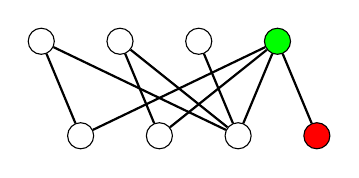
\begin{tikzpicture}[every node/.style={circle, draw}]
      \node[minimum width=3mm] (1) at (0, 0) {};
      \node[minimum width=3mm] (2) at (1, 0) {};
      \node[minimum width=3mm] (3) at (2, 0) {};
      \node[minimum width=3mm] (4) at (-.5, 1.2) {};
      \node[minimum width=3mm] (5) at (.5, 1.2) {};
      \node[minimum width=3mm] (6) at (1.5, 1.2) {};
      \node[minimum width=3mm, fill=green] (7) at (2.5, 1.2) {};
      \node[minimum width=3mm, fill=red] (8) at (3, 0) {};

      \draw[thick] (1) edge (4);
      \draw[thick] (1) edge (7);
      \draw[thick] (2) edge (5);
      \draw[thick] (2) edge (7);
      \draw[thick] (3) edge (4);
      \draw[thick] (3) edge (5);
      \draw[thick] (3) edge (6);
      \draw[thick] (3) edge (7);
      \draw[thick] (8) edge (7);
    \end{tikzpicture}
  \end{figure}\pause

  \bigskip
  會對應到矩陣
$\begin{bmatrix}
  \mid & \mid & & \mid & \mid \\
  \bm{v}_1 & \bm{v}_2 & \cdots & \bm{v}_m & \bm{v}_s \\
  \mid & \mid & & \mid & \mid \\
  0 & 0 & \cdots & 0 & 1 \\
\end{bmatrix}^{\mathsf{T}}$
\end{frame}

\begin{frame}[t]{{\secname}}
  \begin{theorem}
    用 $\text{rank}(A)$ 表示矩陣 $A$ 的維度,則 $\text{rank}(A) = \text{rank}(A^{\sf T})$。
  \end{theorem}

  \pause
  \begin{figure}
    \centering
    \begin{tikzpicture}
      \node (1) at (0, -.3) {$\begin{bmatrix}
        & & & \\
        \bm{v}_1 & \bm{v}_2 & \cdots & \bm{v}_m \\
        & & & \\
      \end{bmatrix}$};

      \node (2) at (5, -.3) {$\begin{bmatrix}
        & & & &\\
        \bm{v}_1 & \bm{v}_2 & \cdots & \bm{v}_m & \bm{v}_s \\
        & & & &\\
      \end{bmatrix}$};

      \node (3) at (0, -3) {$\begin{bmatrix}
        \mid & \mid & & \mid \\
        \bm{v}_1 & \bm{v}_2 & \cdots & \bm{v}_m \\
        \mid & \mid & & \mid \\
        0 & 0 & \cdots & 0 \\
      \end{bmatrix}$} ;

      \node (4) at (5, -3) {$\begin{bmatrix}
        \mid & \mid & & \mid & \mid \\
        \bm{v}_1 & \bm{v}_2 & \cdots & \bm{v}_m & \bm{v}_s \\
        \mid & \mid & & \mid & \mid \\
        0 & 0 & \cdots & 0 & 1 \\
      \end{bmatrix}$};

      \draw (1) edge[-latex, very thick] node[below]{$+1$} (2);
      \draw (3) edge[-latex, very thick] node[above]{$+1$} (4);
      \draw (1) edge[double, double distance=0.5mm, very thick] (3);
      \draw (2) edge[double, double distance=0.5mm, very thick] (4);

      \draw (0, 1.0) node[below]{$\text{rank} = x$};
      \draw (5, 1.0) node[below]{$\text{rank} = x+1$};
      \draw (0, -4) node[below]{$\text{rank} = x$};
      \draw (5, -4) node[below]{$\text{rank} = x+1$};

    \end{tikzpicture}
  \end{figure}
\end{frame}

\begin{frame}{{\secname}}
  加了 $(0, 0, \cdots, 0, 1)$ 以後 $\text{rank}$ 不變,表示 $(0, 0, \cdots, 0, 1)$ 可被
  其他列向量線性組合出 \pause $\implies$ 原本的先手贏。
\end{frame}

\section{Others}

\begin{frame}{{\secname}}
  \begin{problem}[均衡忍者出任務, 2015 ioi-camp]
    請把 $K_n$ 分解成互斥的三角形,其中 $n = 2^k - 1$。
  \end{problem}

  \begin{figure}
    \centering
    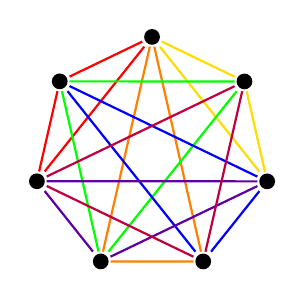
\begin{tikzpicture}
      \foreach \d [count=\xi] in {90, 141.42, ..., 398.57} {
        \fill (\d:1.5cm) node(\xi){} circle (1mm);
      }

      \draw[thick, red] (1) -- (2) -- (3) -- (1);
      \draw[thick, orange] (1) -- (4) -- (5) -- (1);
      \draw[thick, yellow!80!orange] (1) -- (6) -- (7) -- (1);
      \draw[thick, green] (2) -- (4) -- (7) -- (2);
      \draw[thick, blue] (2) -- (5) -- (6) -- (2);
      \draw[thick, blue!50!purple] (3) -- (4) -- (6) -- (3);
      \draw[thick, purple] (3) -- (5) -- (7) -- (3);
    \end{tikzpicture}
  \end{figure}
\end{frame}
\begin{frame}{{\secname}}
  如果可以找到函數 $f(x, y)$ 使得 $x \neq y \implies f(x, y) \neq x, y$ 且 $f(x, f(x, y)) = y,\ f(f(x, y), y) = x$,
  我們就做完了!
\end{frame}

\begin{frame}{{\secname} -- Pr\"{u}fer sequence}
  \begin{problem}
    求 $n$ 個有編號的點可以形成多少種不同的樹。
  \end{problem} \pause

  \bigskip
  答案是 $n^{n-2}$。
\end{frame}

\begin{frame}{{\secname} -- Pr\"{u}fer sequence}
  每次找葉子中編號最小的點 $u$,假設他連出去的邊是 $(u, v)$,
  就記下 $v$ 的編號,並把 $v$ 和邊 $(u, v)$ 從圖上刪除。重複直到圖上就只剩一個點了。
  \pause

  \begin{figure}
    \centering
    \begin{tikzpicture}[every node/.style={draw, circle}, scale=0.8]
      \useasboundingbox (-2, -2) rectangle (3, 3);
      %\node (1) at (-.8, -1.3) {$1$};
      \node<2> (3) at (2.6, .1) {$3$};
      \node<2-3> (5) at (-1.4, .5) {$5$};
      \node<2-4> (4) at (0, 0) {$4$};
      \node<2-5> (2) at (1.4, 1.3) {$2$};
      \node (6) at (2.6, 2.4) {$6$};

      \node<2>[fill=black!20] (1) at (-.8, -1.3) {$1$};
      \node<3>[fill=black!20] (3) at (2.6, .1) {$3$};
      \node<4>[fill=black!20] (5) at (-1.4, .5) {$5$};
      \node<5>[fill=black!20] (4) at (0, 0) {$4$};
      \node<6>[fill=black!20] (2) at (1.4, 1.3) {$2$};

      \draw<2> (1) edge[thick] (4);
      \draw<2-3> (3) edge[thick] (2);
      \draw<2-4> (4) edge[thick] (5);
      \draw<2-5> (2) edge[thick] (4);
      \draw<2-6> (2) edge[thick] (6);
    \end{tikzpicture}
  \end{figure}

  \[ \visible<2->{4}\visible<3->{\to 2} \visible<4->{\to 4} \visible<5->{\to 2} \visible<6->{\to 6} \]
\end{frame}

\begin{frame}{{\secname} -- 構造}
  \begin{problem}[均衡忍者出任務, 2015 ioi-camp]
    請把 $K_n$ 分解成互斥的三角形,其中 $n = 2^k - 1$。
  \end{problem}

  \begin{figure}
    \centering
    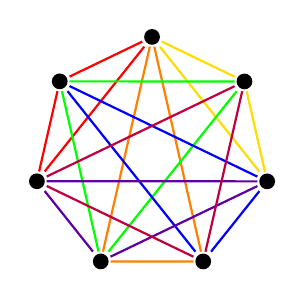
\begin{tikzpicture}
      \foreach \d [count=\xi] in {90, 141.42, ..., 398.57} {
        \fill (\d:1.5cm) node(\xi){} circle (1mm);
      }

      \draw[thick, red] (1) -- (2) -- (3) -- (1);
      \draw[thick, orange] (1) -- (4) -- (5) -- (1);
      \draw[thick, yellow!80!orange] (1) -- (6) -- (7) -- (1);
      \draw[thick, green] (2) -- (4) -- (7) -- (2);
      \draw[thick, blue] (2) -- (5) -- (6) -- (2);
      \draw[thick, blue!50!purple] (3) -- (4) -- (6) -- (3);
      \draw[thick, purple] (3) -- (5) -- (7) -- (3);
    \end{tikzpicture}
  \end{figure}
\end{frame}
\begin{frame}{{\secname} -- 構造}
  如果可以找到函數 $f(x, y)$ 使得 $x \neq y \implies f(x, y) \neq x, y$ 且 $f(x, f(x, y)) = y,\ f(f(x, y), y) = x$,
  我們就做完了!\pause

  \bigskip
  事實上,只要 $n \equiv 1, 3 \pmod{6}$ 就會有解!
\end{frame}

\begin{frame}{{\secname} -- 構造}
  \begin{problem}[Graph Factorization, ASC 35 pF]
    請把 $K_{2n}$ 分解成 $2n-1$ 個互斥的完美匹配。
  \end{problem}

  \begin{figure}
    \centering
    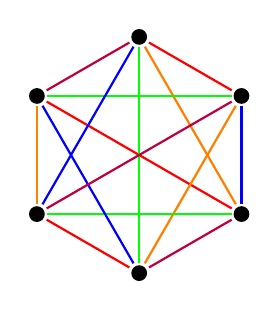
\begin{tikzpicture}
      \foreach \d [count=\xi] in {90, 150, ..., 390} {
        \fill (\d:1.5cm) node(\xi){} circle (1mm);
      }
      \draw[thick, red] (1) -- (6);
      \draw[thick, red] (2) -- (5);
      \draw[thick, red] (3) -- (4);
      \draw[thick, orange] (1) -- (5);
      \draw[thick, orange] (6) -- (4);
      \draw[thick, orange] (2) -- (3);
      \draw[thick, green] (1) -- (4);
      \draw[thick, green] (5) -- (3);
      \draw[thick, green] (6) -- (2);
      \draw[thick, blue] (1) -- (3);
      \draw[thick, blue] (4) -- (2);
      \draw[thick, blue] (5) -- (6);
      \draw[thick, purple] (1) -- (2);
      \draw[thick, purple] (3) -- (6);
      \draw[thick, purple] (4) -- (5);
    \end{tikzpicture}
  \end{figure}
\end{frame}

\begin{frame}{{\secname} -- 機率}
  \begin{problem}[Graph Game, Codeforces 235D]
    現在有一個遊戲:一開始的分數是 $0$,並且有一個 $n$ 個點的樹,
    每次從剩下的點中隨機且等機率的選出一個點 $v$,並把分數加上 $v$ 所在的
    連通塊的大小,且把 $v$ 和與 $v$ 相鄰的邊全部刪掉。一直進行到圖上沒有點為止,
    問你得到的分數的期望值。
  \end{problem}\pause

  \bigskip
  機率有關的題目通常會玩一個梗:
  \begin{lemma} \vspace{-1em}
    \[ \Expect[X + Y] = \Expect[X] + \Expect[Y] \]
  \end{lemma}
\end{frame}

\begin{frame}{{\secname}}
  \begin{figure}
    \centering
    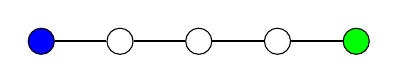
\begin{tikzpicture}[every node/.style={circle, draw, minimum width=3mm}]
      \node(1) at (0, 0) {};
      \node(2) at (1, 0) {};
      \node[fill=green] (3) at (2, 0) {};
      \node(4) at (-1, 0) {};
      \node[fill=blue] (5) at (-2, 0) {};
      \draw (1) edge[thick] (2);
      \draw (3) edge[thick] (2);
      \draw (1) edge[thick] (4);
      \draw (5) edge[thick] (4);
    \end{tikzpicture}
  \end{figure} \pause

  \medskip
  不過原本的題目其實是一棵水母。

  \medskip
  \begin{figure}
    \centering
    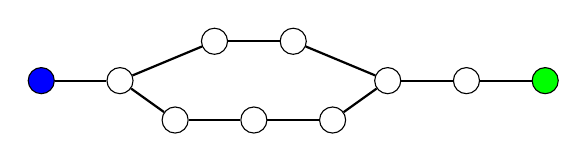
\begin{tikzpicture}[every node/.style={circle, draw, minimum width=3mm}]
      \node(1) at (0.2, 0) {};
      \node(2) at (1.2, 0) {};
      \node[fill=green] (3) at (2.2, 0) {};
      \node(4) at (-0.5, -0.5) {};
      \node(5) at (-1.5, -0.5) {};
      \node(6) at (-2.5, -0.5) {};
      \node(7) at (-1, 0.5) {};
      \node(8) at (-2, 0.5) {};
      \node(9) at (-3.2, 0) {};
      \node[fill=blue] (10) at (-4.2, 0) {};
      \draw (1) edge[thick] (2);
      \draw (3) edge[thick] (2);
      \draw (1) edge[thick] (4);
      \draw (5) edge[thick] (4);
      \draw (5) edge[thick] (6);
      \draw (9) edge[thick] (6);
      \draw (9) edge[thick] (10);
      \draw (1) edge[thick] (7);
      \draw (8) edge[thick] (7);
      \draw (8) edge[thick] (9);
    \end{tikzpicture}
  \end{figure}
\end{frame}


\begin{frame}{{\secname}}
  \begin{problem}
    給你許多點 $(x_1, y_1), (x_2, y_2), \cdots, (x_n, y_n)$,請找一個線性函數 $f$ 使得
    $\sum (f(x_i) - y_i)^2$ 最小。
  \end{problem}\pause

  \bigskip
  \begin{problem}
    給你許多點 $\bm{x}_1, \bm{x}_2, \cdots, \bm{x}_n$,請找一條線 $l$ 使得
    $\sum d(\bm{x}_i, l)^2$ 最小。
  \end{problem}
\end{frame}

\end{document}

